\problemname{The Innovative Water Clock}

Simon has been reading about water clocks in school - water pours into
a vessel at a constant rate, so that the amount of water in the vessel
indicates the amount of time that has passed.  He has decided to make
such a clock, but thinks that the traditional method of a simple
cylinder with lines up the side to note the passage of time is too
boring.  Instead, he would like his containers to fill up in
interesting patterns.  His clocks will be rectangular (when viewed
from the side) and with some internal walls so that different areas
(grid cells) of the clock will fill up at different times.  He will
give you a picture of the side view of the clock he would like to
build.  In his clocks, water will be poured in at the rate of one grid
cell per minute, and each number given represents which minute that
particular square will become completely full.  Here is an example:

\begin{center}
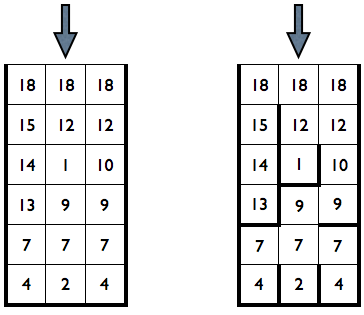
\includegraphics[width=4in]{water-example.png}
\end{center}

On the left is Simon's specification.  On the right, we can see the
necessary walls.  After 1 minute, the cell with the 1 will be full.
After 1 more minute (2 minutes total), the water overflowing the ``1''
cell will fill up the cell marked ``2''.  The two cells marked ``4''
will fill up at the same time, so they both fill after 2 more minutes
(4 minutes total), and so on.  Of course, Simon doesn't want to have
to build more walls than necessary, so you must find the smallest
set of walls that satisfies his specification.

\section*{Input}
  The first line contains $k$, the number of input instances.  The
  first line of each input instance contains three numbers: $m$, the
  number of rows of the clock, $n$, the number of columns of the
  clock, and $c$, the column into which the water source will pour
  ($c=1$ represents the left-most column), with $m\times n < 40$.
  This is followed by $m$ lines, each containing $n$ integers
  representing the required fill times for the corresponding cell of
  the clock.

\section*{Output}
  The output will consist of the solution for each input instance, in
  order, separated by a single blank line.  For each input instance,
  the output will consist of $2m$ lines.  Each odd line represents the
  cells of the clock (represented with {\tt 'o'}) and, if present,
  the vertical wall segments (represented with {\tt '|'}) including
  those on the outside of the clock.  If no vertical wall is present
  in a location, a space should be printed instead.  Each even line
  represents the boundary between two rows of cells.  This should
  consist of spaces except where a horizontal wall segment is present,
  which should appear as a hyphen ({\tt '-'}).
